\chapter{Gaseous flow in BIMER multipoint injector}
	\label{ch9:bimer_test_bench_and_aero}

\section{Introduction}

The jet in crossflow atomizer from the previous chapters is an academic test case of fuel representative of LPP systems. Its study is of interest for aeronautical gas turbines since it uses kerosene as injected liquid and it has been tested in a high-pressure environment. Yet, its

The fact that the injected liquid is kerosene is 

Here we describe the aerodynamic simulations performed with BIMER. Two operating points are simulated:



\section{Experimental setup}

Dodecane properties are shown in Table \ref{tab:dodecane_properties}

\begin{table}[!h]
\centering
\caption{Physical properties of dodecane fuel.}
\begin{tabular}{|c|c|c|}
\hline
$\rho$ [kg m$^{-3}]$   & $\mu$ [Pa s]   & $\sigma$ [N/m]  \\
\hline
750 & $1.36 \cdot 10^{-3}$ & $22 \cdot 10^{-3}$ \\
\hline
\end{tabular}
\label{tab:dodecane_properties}
\end{table}


\section{Choice of operating points}

In first place, the 

Gaseous flow simulations of BIMER have been performed for two operating conditions tested experimentally, with the purpose of using one condition for validation and the other for application:

\begin{itemize}

	\item \textbf{Validation} of the gaseous simulations is performed with the operating point tested experimentally by \citeColor[providakis_etude_2013], since this one presents data on the non-reactive aerodynamic field. The simulations are also compared to numerical results obtained for this same operating condition by \citeColor[cheneau_etude_2019]. 
	
	\item \textbf{Application} to the setup condition tested by \citeColor[renaud_high-speed_2015]. This study shows data on non-reactive spray characteristics, and hence it will be used as the application case to run the full workflow formerly introduced in Chapter \ref{ch:sli_development}. It is, nowever, not used for validating the gaseous simulations since it does not present pertinent data.

\end{itemize}

Both ope

\begin{table}[!h]
\centering
\caption{Operating points for performing non-reactive gaseous simulations}
\begin{tabular}{|c|c|c|c|c|c|}
\hline
Operating condition   &  $\dot{m}_g$ [g s$^{-1}$] & $T_g$ [K] & $\rho_g$ [kg m$^{-3}]$  & $\mu_g$ [Pa s] & $p$ [Pa]  \\
\hline
\hline
Validation \citepColor[providakis_etude_2013] & 53 & 473 & 0.746089 & $2.571 \cdot 10^{-5}$ & 101300 \\
\hline
Application \citepColor[renaud_high-speed_2015] & 43.1 & 433 & 0.816382 & $2.3911 \cdot 10^{-5}$ & 101300 \\
\hline
\end{tabular}
\label{tab:gaseous_operating_points_BIMER}
\end{table}

\begin{table}[!h]
\centering
\caption{BIMER operating point to validate non-reactive gaseous simulations tested by \citeColor[providakis_etude_2013]}
\begin{tabular}{|c|c|c|c|c|}
\hline
$\dot{m}_g$ [g s$^{-1}$] & $T_g$ [K] & $\rho_g$ [kg m$^{-3}]$  & $\mu_g$ [Pa s] & $p$ [Pa]  \\
\hline
\hline
53 & 473 & 0.746089 & $2.571 \cdot 10^{-5}$ & 101300 \\
\hline
\end{tabular}
\label{tab:gaseous_operating_point_Providakis}
\end{table}



\section{Numerical setup}

\section{Mesh independence study}

\section{Validation of gaseous field}

Results are contained here: $Ongoing - BIMER - postprocessing - aero$. They were discussed in the pilotage of 16 March 2021.

%Show nice streamlines (Fig. 6.4 Esclapez-1) and PVC. It would be nice to compare them for both operating conditions

\begin{figure}[h!]
	\centering
	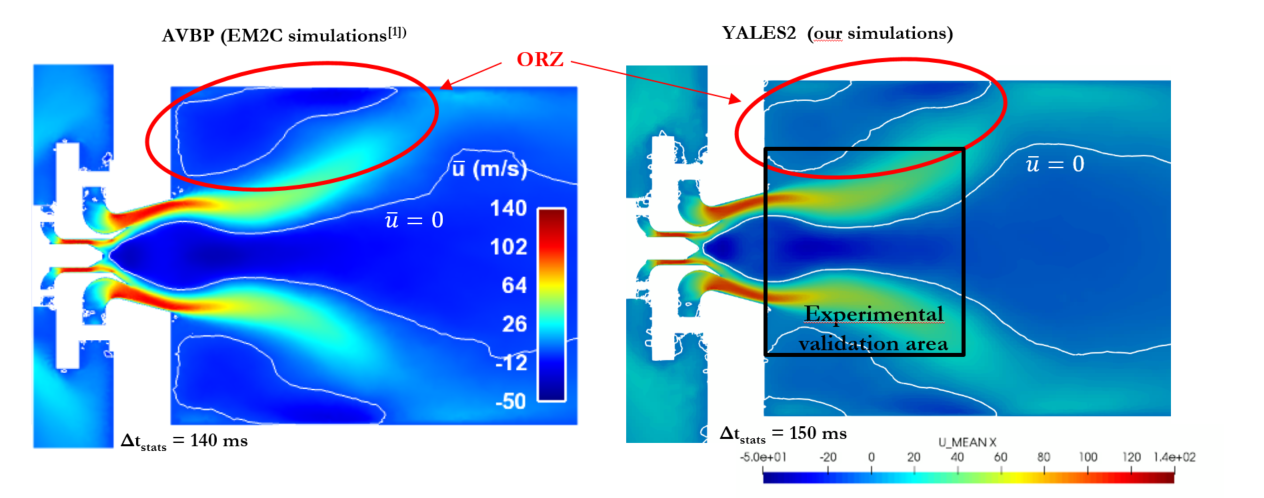
\includegraphics[scale=0.7]{./part3_applications/figures_aero/quantitative_view_mean_velocity_field}
	\caption{Mean velocity field .}
	\label{fig:quantitative_view_mean_velocity_field}
\end{figure}


\subsection{Qualitative validation}


See Figure \ref{fig:validation_qualitative_u}: \ref{fig:validation_qualitative_u_mean} and \ref{fig:validation_qualitative_u_rms}.


\begin{figure}
\centering
\begin{subfigure}[b]{1.0\textwidth}
	\centering
   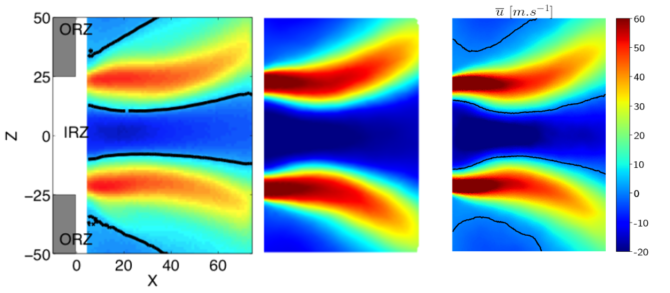
\includegraphics[scale=1.0]{./part3_applications/figures_aero/validation_qualitative_u_mean}
   \caption{Mean axial velocity}
   \label{fig:validation_qualitative_u_mean} 
\end{subfigure}
\begin{subfigure}[b]{1.0\textwidth}
	\centering
   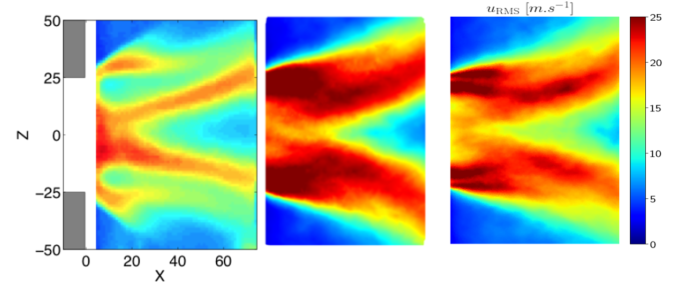
\includegraphics[scale=1.0]{./part3_applications/figures_aero/validation_qualitative_u_rms}
   \caption{RMS axial velocity}
   \label{fig:validation_qualitative_u_rms}
\end{subfigure}
\caption{Fields of axial velocity in enclosed region from Figure \ref{fig:quantitative_view_mean_velocity_field}. \textsl{Left}: experimental results. \textsl{Center}: numerical results obtained by \citeColor[cheneau_etude_2019]. \textsl{Right}: results from present work.}
\label{fig:validation_qualitative_u}
\end{figure}

\begin{figure}
\centering
\begin{subfigure}[b]{1.0\textwidth}
	\centering
   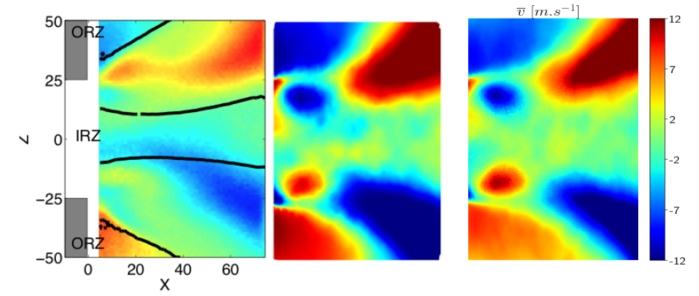
\includegraphics[scale=1.0]{./part3_applications/figures_aero/validation_qualitative_v_mean}
   \caption{Mean vertical velocity}
   \label{fig:validation_qualitative_v_mean} 
\end{subfigure}
\begin{subfigure}[b]{1.0\textwidth}
	\centering
   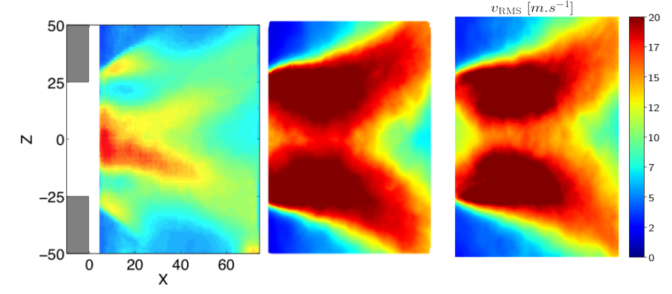
\includegraphics[scale=1.0]{./part3_applications/figures_aero/validation_qualitative_v_rms}
   \caption{RMS vertical velocity}
   \label{fig:validation_qualitative_v_rms}
\end{subfigure}
\caption{Fields of vertical velocity in enclosed region from Figure \ref{fig:quantitative_view_mean_velocity_field}. \textsl{Left}: experimental results. \textsl{Center}: numerical results obtained by \citeColor[cheneau_etude_2019]. \textsl{Right}: results from present work.}
\label{fig:validation_qualitative_v}
\end{figure}





\subsection{Quantitative validation}

\section{Application point}

\section{Conclusion}

%\section{Validation (Providakis 2013)}
%
%
%\subsection{Quantitative data}
%
%\subsection{Qualitative data}
%
%\section{Application (Renaud 2015)}
%
